The fixed baseline protocol comprises 1,260 main cells and 720 supplementary cells. It uses exact Gaussian and Gaussian-mixture factor scores, isolating random-weight effects from learned-model approximation. Baseline benchmark cells use 8,192 particles, $M=4$, $G\in\{16,64\}$, $d\in\{1,8\}$, $K\in\{128,512,2048\}$, and five random seeds. The reverse-time grid is $u_k=20(1-k/K)^2$, the initial distribution is $\Normal(0,I)$, and $\kappa=1$. The finite-$U$ initialization is an approximation to the exact compositional path. Reference marginals are computed by numerical quadrature on 65,537 points in $[-12,12]$.

The main comparison includes full-factor weighting, an unweighted composed drift, plug-in weighting, unbiased quadratic weighting, a paired cumulant correction, and two moment-matched Gaussian control variants. The supplementary benchmark evaluates tail control and its paired correction on both mixture families. Paired corrections use two independent batches and the positive weight $\exp\{h(\widehat g_1+\widehat g_2)/2-h^2(\widehat g_1-\widehat g_2)^2/8\}$, with the averaged drift; they therefore require twice as many sampled factor evaluations. This correction is an empirical ablation, with no claim of exact exponential unbiasedness.

For the one-step example in \eqref{eq:counterexample}, the supplementary study uses $P\in\{1{,}024,16{,}384,262{,}144,1{,}048{,}576\}$, $M\in\{2,4,8,16,32\}$, and 20 seeds, together with the full-factor update. We retain histograms and the 1,024 largest normalized particle weights for each one-step cell. The benchmark retains complete particle arrays and reference distributions.

All 1,980 baseline cells completed on SCNet RTX 3080 GPUs. We verified the source versions, 13,506 recovered file hashes, all 40 task exit records, and the complete cell configuration lists. Benchmark metrics were recomputed using independent numerical routines. Adaptive quadrature over the real line also verified all 54 reference coordinates, including analytic Gaussian checks. A separately frozen extension adds 1,080 oracle sampling cells and 1,000 learned-density sampling cells, with five complete network trainings (Appendix~\ref{app:extension-protocol}).

\subsection{Local error decreases while the normalizer remains infinite}
Figure~\ref{fig:one-step} shows the one-step experiment. At $P=1{,}048{,}576$, increasing $M$ from 2 to 32 reduces mean potential MSE from $0.46798$ to $0.01857$, approximately a factor of 25. The median ESS fraction rises from $0.000424$ to $0.932706$. Nevertheless, \eqref{eq:counterexample} gives an infinite population normalizer for both batch sizes and every intermediate finite $M$.

For $M=32$, the empirical mean log normalizer is $0.126047$ with standard deviation $0.000259$ across 20 seeds. The full-factor result is $0.122030\pm0.000234$, close to its exact value $0.122049$. No nonintegrable batch was sampled in these 20 runs of $1{,}048{,}576$ particles with $M=32$. The all-strongest event alone has probability $4^{-32}\approx5.42\times10^{-20}$ per batch. Its absence in this finite experiment cannot establish existence of the population target. For $M=2$, the median estimated log normalizer rises from $0.270$ at $P=1{,}024$ to $0.484$ at $P=1{,}048{,}576$, accompanied by severe ESS loss. The proof supplies the divergence result; these finite observations illustrate why it can be visible at small $M$ and inconspicuous at larger $M$.

\begin{figure}[t]
 \centering
 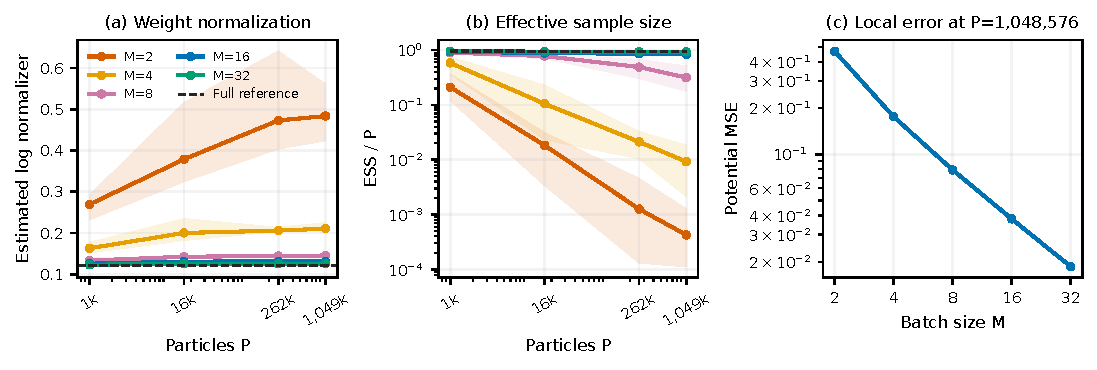
\includegraphics[width=\linewidth]{figures/one_step.pdf}
 \caption{One-step Gaussian counterexample. Panels (a,b) show medians and interquartile ranges over 20 seeds. The dashed reference is the exact full-factor log normalizer in (a) and the empirical full-factor ESS fraction in (b). Panel (c) shows mean potential MSE with one standard deviation at $P=1{,}048{,}576$. Every subsampled curve has an infinite population normalizer.}
 \label{fig:one-step}
\end{figure}

\subsection{Certificates across the benchmark grid}
Appendix Table~\ref{tab:certificates} reports validity over the 12 configurations per family, formed by two group counts, two dimensions, and three time grids. Seeds do not change a certificate. Raw plug-in, unbiased, and paired estimators fail all Gaussian and ordinary-mixture configurations. Moment matching makes the Gaussian estimator exact, but does not certify any ordinary-mixture configuration. Tail matching recovers the full-factor strict domain in both mixture families. The complete configuration-level grid is provided in Appendix~\ref{app:full-results}.

The full-factor discretization also fails for $G=64,K=128$ in the Gaussian and ordinary-mixture families. Its Gaussian denominator first becomes negative at step 100, reaching approximately $-0.003111$. Yet the observed mean marginal W1 is only $0.0141$ in one dimension and $0.0176$ in eight dimensions. Thus a small endpoint sample discrepancy can coexist with an undefined population update even before subsampling. For finite Gaussian configurations, exact weighted-Euler moment recursion separates time error from particle error: at $G=64,K=2048$, the population W1 is approximately $0.000493$, while the eight-dimensional finite-particle mean marginal W1 is $0.0149$.

\subsection{A finite domain does not guarantee accurate or faster inference}
Figure~\ref{fig:accuracy-time} and Table~\ref{tab:matched} compare actual sampler time and endpoint error. For the difficult eight-dimensional ordinary mixture with $G=64,K=512$, all weighted methods have substantial sampling error. Full-factor W1 is $0.881\pm0.372$, tail control is $1.004\pm0.327$, and paired tail control is $1.358\pm0.188$. Their mean total-variation errors over the 256 coordinate-sign patterns are respectively $0.961$, $0.975$, and $0.998$, confirming poor joint-mode coverage. The paired moment control has lower marginal W1, $0.456\pm0.228$, despite an infinite population normalizer. These outcomes demonstrate that finite integrability, marginal accuracy, and joint coverage are distinct properties.

\begin{figure}[t]
 \centering
 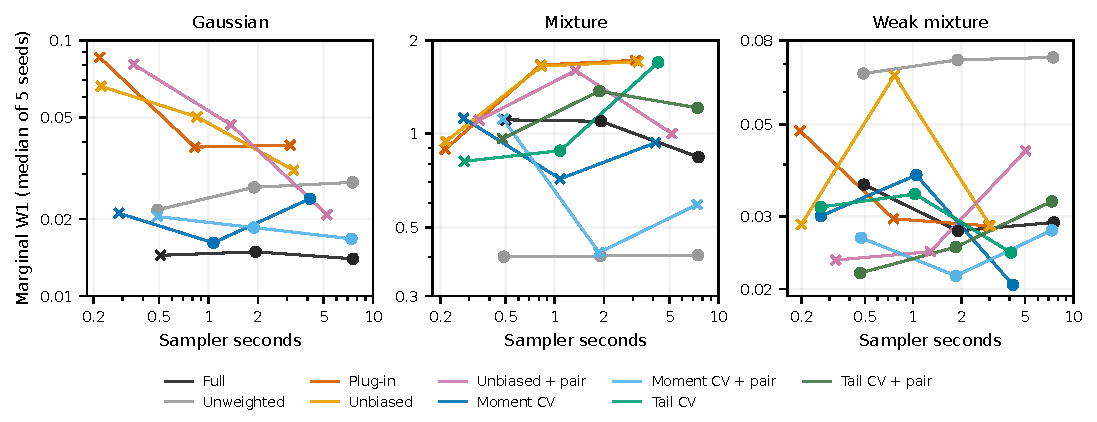
\includegraphics[width=\linewidth]{figures/accuracy_time.pdf}
 \caption{Observed error versus recorded sampler time at $G=64,d=8$, with $K\in\{128,512,2048\}$. Each point is a median over five seeds. Circles denote finite population normalizers and crosses denote infinite ones. Lines connect a method's three time grids and are not fitted performance models.}
 \label{fig:accuracy-time}
\end{figure}

On the weak mixture, paired tail control yields W1 $0.025\pm0.005$, compared with $0.028\pm0.007$ for full weighting, at nearly the same recorded sampler time. Unpaired tail control uses 16 times fewer nonlinear particle--factor evaluations and about $1.86$ times less sampler time, but its W1 rises to $0.043\pm0.026$. We therefore make no general speed--accuracy superiority claim. Gaussian full and exact-control results, complete seed-level metrics, and additional joint diagnostics are retained in the artifacts.

\subsection{Without replacement: batch size changes the finite domain}\label{sec:without-replacement-results}
The prefix/suffix certificate permits an exhaustive scan over batch sizes without enumerating subsets. Table~\ref{tab:batch-thresholds} reports the smallest finite batch size among all $2\le M\le G$ for the benchmark tails. This separate deterministic calculation comprises 936 configurations and agrees with direct subset enumeration in nine smaller cross-checks. The ordinary mixture shares the Gaussian component variances, and dimensions one and eight give identical thresholds here. All larger batch sizes are finite in each displayed case with a finite threshold; this observed ordering is not claimed as a general monotonicity theorem. At $G=64,K=512$, switching from replacement to a uniform subset of size four remains below either family's threshold. Thus removing repeated indices changes the certificate but does not by itself make a small batch valid.

\begin{table}[t]
 \centering
 \caption{Smallest certified finite without-replacement batch size, with $U=20$, $\kappa=1$ and initial variance one. A dash means no finite batch exists, including $M=G$. The mixture rows use the strict tail certificate.}
 \label{tab:batch-thresholds}
 \begin{tabular}{lrccc}
 \toprule
 Tail family & $G$ & $K=128$ & $K=512$ & $K=2048$\\
 \midrule
 Gaussian / ordinary mixture & 16 & 13 & 12 & 12\\
 Gaussian / ordinary mixture & 64 & -- & 60 & 59\\
 Weak mixture & 16 & 3 & 2 & 2\\
 Weak mixture & 64 & 22 & 18 & 17\\
 \bottomrule
 \end{tabular}
\end{table}

